\section{Density Operator Formalism - 密度运算符}
When using quantum systems for \impt{processing information} (i.e. ``doing quantum information processing''), it is necessary to model \impt{missing, incomplete, subjective knowledge} about a state in a quantum system. Some examples are quantum key exchange (imperfect state preparation), errors during a quantum computation (imperfect measurements), and inaccurate model of a Hamiltonian. \par
Classically, if we have perfect knowledge about a state of a system, say an $n$-bit string, the state is a specific bit string $\vec{b} \in \{0, 1\}^n$. However, with imperfect or subjective knowledge, a ``state'' is a probability distribution over $\{0, 1\}^n$. The probability map would be:
$$\Prob{\vec{b}}: \vec{b} \in \{0, 1\}^n \to [0,1]$$
where we satisfy $\sum \Prob{\vec{b}} = 1$ and $\Prob{\vec{b}} \ge 0$. \par
In a quantum formalism, a state is a normalized vector $\ketpsi \in \hilbert$. The corresponding imperfect representation would be \impt{density operators}. \par
Suppose a quantum system associated with $\hilbert$ is prepared according to:
\begin{quote}
    1. Generate a number $i \in \{1, \dots, n\}$ with probability $\text{Pr}_i$, where $\text{Pr} \ge 0$ and $\displaystyle \Sum{i = 1}{n} \text{Pr}_i = 1$. \\
    2. Prepare the quantum state $\ket{\psi_i} \in \hilbert$, where $\{\ket{\psi_i}_{i = 1}^n\}$ is an arbitrary set of quantum states.
\end{quote}
We now wish to know how we can efficiently describe this ``state'', if we do not know $i$. In words, we can say: state $\ket{\psi_i}$ with probability $\text{Pr}_i$; or mathematically, as \impt{probability mixtures}: $\{(\text{Pr}_i, \ket{\psi_i})\}_{i=1}^n$. \par
We can find a more efficient mathematical object that captures \impt{all relevant information} of a probability mixture, where all relevant information is \impt{the probability of measurement outcomes}. We then calculate the outcome probability of a measurement with respect to projection operators $\{\Pi_x\}_x$:
\begin{align*}
    \Prob{x: \{(\text{Pr}_i, \ket{\psi_i})\}} &= \Sum{i = 1}{n} \Prob{\ket{\psi_i}} \times \Prob{x \mid \ket{\psi_i}} \\
    &= \Sum{i=1}{n} \text{Pr}_i \ev{\Pi_x}{\psi_i} \\
    &= \Sum{i=1}{n} \text{Pr}_i \tr(\Pi_x \dyad{\psi_i}) \\
    &= \tr(\Pi_x \cdot \Sum{i=1}{n} \text{Pr}_i \dyad{\psi_i})
\end{align*}
This result comes from the property of the trace. Consider the orthonormal basis of $\Pi_x \dyad{\psi_i}$ to be $\{\ket{\phi_k}\}_{k=1}^d$, we choose $\ket{\phi_1} = \ket{\psi_i}$ and complete the basis accordingly, we then have:
\begin{align*}
    \tr(\Pi_x \dyad{\psi_i}) &= \Sum{k=1}{d} \mel{\phi_k}{\Pi_x}{\psi_i}\braket{\psi_i}{\phi_k} \\
    &= \mel{\phi_1}{\Pi_x}{\psi_i} \\
    &= \ev{\Pi_x}{\psi_i}
\end{align*}
\begin{definition}
    Given a Hilbert space $\hilbert$, and prepare a number of states $\{\ket{\psi_i}\}_{i=1}^n$ with each state having the probability of $p_i$, then, the \uimpt{density operator} that represent this ``state'' is
    $$\rho = \Sum{i=1}{n} p_i \dyad{\psi_i}$$
\end{definition}
Note that the density operator is a convex linear combination of projectors, hence $\rho: \hilbert \to \hilbert$ is a linear operator. Some properties of the density operator include:
\begin{quote}
    1. $\rho$ is Hermitian \\
    2. $\rho \ge 0$ is semi-definite: $\ev{\rho}{\phi} = \sum p_i \braket{\phi}{\psi_i}\braket{\psi_i}{\phi} = \sum p_i \abs{\braket{\phi}{\psi_i}}^2 \ge 0$. \\
    3. $\tr(\rho) = 1$: $\tr(\Sumi{i}p_i \dyad{\psi_i}) = \Sumi{i}p_i \tr(\dyad{\psi_i}) = \Sumi{i}p_i = 1 $
\end{quote}
\begin{theorem}
    Any Hermitian, positive semi-definite, unit trace operator $\sigma$ can be written as:
    $$\sigma = \Sumi{i} q_i \dyad{\phi_i}$$
    where $\{q_i\} \subseteq \R$ and $\{\ket{\phi_i}\}$ is an orthonormal basis. \\
    $\sigma$ corresponds to (can be interpreted as) the probability mixture:
    $$\{(q_i, \ket{\phi_i})\}_i$$
    This is not unique.
\end{theorem}
This is essentially the spectral decomposition of a density operator. \\
The set of density operators (a.k.a ``quantum states'') of a system associated to $\hilbert$ is:
$$\mathcal{S}(\hilbert) = \{\rho \text{ is a linear operator on }\hilbert \mid \rho \ge 0, \conjt{\rho} = \rho, \tr(\rho) = 1\}$$
For density operators, $\rho \in \mathcal{S}(\hilbert)$ does not specify a unique probability mixture, which inherently tells us that probability mixtures are redundant.
\begin{definition}
    The density operator $\rho$ is \uimpt{pure}, if there exists $\ketphi \in \hilbert$, $\rho = \dyad{\phi}$. This uniquely defines a probability mixture. If $\rho$ is not pure, it is \uimpt{mixed}.
\end{definition}
A mixture of mixed states is also a mixed state. That is, consider a probability mixture $\{(q_i, \sigma_i)\}$, where $\sigma_i \in \mathcal{S}(\hilbert)$, the corresponding density operator:
$$\rho = \sum q_i \cdot \sigma_i$$
is also a mixed state. 
\begin{definition}
    $\rho$ is \uimpt{maximally mixed} if $\rho = \frac{\id}{\dim(\hilbert)}$
\end{definition}
This is essentially a uniform distribution in a classical sense. \\
Notice that for composite system $\hilbert_A \otimes \hilbert_B$, the set of density operators are defined:
$$\mathcal{S}(\hilbert_A \otimes \hilbert_B) = \{\rho \text{ is a linear operator on }\hilbert \mid \rho \ge 0, \conjt{\rho} = \rho, \tr(\rho) = 1\}$$
$$\mathcal{S}(\hilbert_A \otimes \hilbert_B) \ne \mathcal{S}(\hilbert_A) \otimes \mathcal{S}(\hilbert_B)$$
as $\mathcal{S}$ is not a linear space. \\
To compare the vector formalism and the density operator formalism, refer to the following table:
\begin{center}
    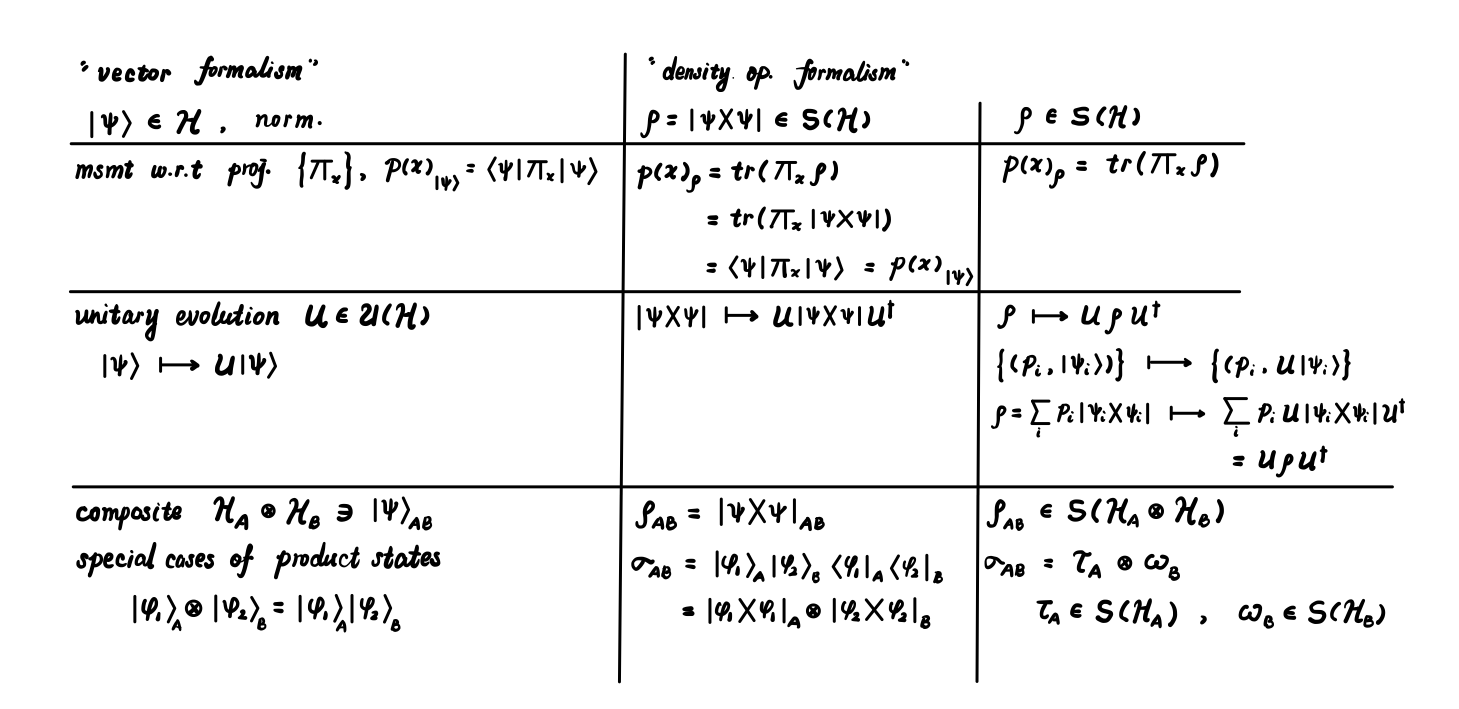
\includegraphics[scale = 0.625]{vec-rho.png}
\end{center}

\subsection{Partial Trace}
Consider a bipartite state $\rho_{AB} \in \mathcal{S}(\hilbert_A \otimes \hilbert_B)$, we want to find a way (an operation) to ``reduce'' $\rho_{AB}$ to a ``local state'', say $\rho_A \in \mathcal{S}(\hilbert_A)$, such that $\rho_A$ captures all physical properties of the $A$ system. Mathematically, this is finding an operation that maps $\rho_{AB} \mapsto \rho_A$ such that all projective measurements on $A$ $\{\Pi_x\}$:
$$\Prob{x}_{\rho_{AB}} = \tr((\Pi_x \otimes \id)\rho_{AB}) = \tr(\Pi_x \rho_A) = \Prob{x}_{\rho_A}$$
Recall that any linear operator $M_{AB}$ on $\hilbert_A \otimes \hilbert_B$ can be written as:
$$M_{AB} = \Sumi{k} S_k \otimes T_k$$
Then,
\begin{definition}
    The \uimpt{partial trace} over $B$ when $\hilbert = \hilbert_A \otimes \hilbert_B$ is map where:
    \begin{align*}
        \tr_B: \{\text{linear operator on the composite system}\} &\to \{\text{linear operator on }\hilbert_A\} \\
        M_{AB} = \Sumi{k} S_k \otimes T_k &\mapsto \Sumi{k} S_k \cdot \tr(T_k)
    \end{align*}
\end{definition}
If $\rho_{AB} \in \mathcal{S}(\hilbert_A \otimes \hilbert_B)$, then $\rho_A = \tr_B(\rho_{AB}) \in \mathcal{S}(\hilbert_A)$ is also a vaild density operator. The partial trace is essentially a map that maps an \impt{endomorphism of the composite system} to an \impt{endomorphism of the local system}. The local trace $\rho_A := \tr_B(\rho_{AB})$ is called the marginal (compare to the marginals of probability distributions)/reduced/local state. Applying the partial trace $\tr_B$, we say ``\impt{we trace out B}''. Different global states $\rho_{AB}$ can lead to the same local state. Marginals of pure states are not necessarily pure. \\
Recall that our goal was to find the ``reduction'', and we claim the partial trace does the job. To start with, consider these two elementary properties of the partial trace:
\begin{quote}
    1. $\tr(M_{AB}) = \tr(\tr_B(M_{AB}))$. \\
    2. $\tr_B((N_A \otimes \id_B)M_{AB}) = N_A \tr_B(M_{AB})$
\end{quote}
Then, 
\begin{align*}
    \tr((\Pi_x \otimes \id)\rho_{AB}) &= \tr(\tr_B((\Pi_x \otimes \id)\rho_{AB})) \\
    &= \tr(\Pi_x \tr_B(\rho_{AB})) \\
    &= \tr(\Pi_x \rho_A)
\end{align*}
This is the unique operation that satisfies this relation for all states $\rho_{AB}$ and all local measurements $\{\Pi_x\}_x$. Thus, we can consider a commutative diagram that relate the composite system and the local system by considering a local unitary evolution:
\begin{center}
    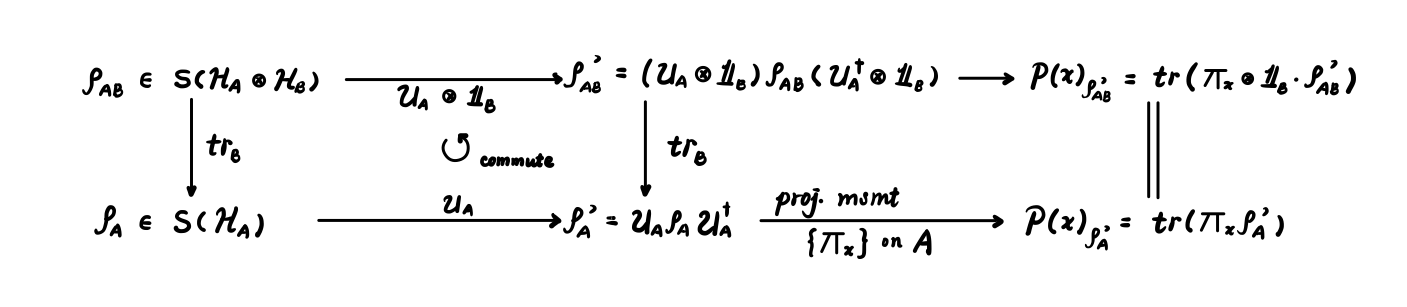
\includegraphics[scale = 0.625]{partial-trace.png}
\end{center}
Now, we are able to reduce the composite system to a local system, we wish to know whether or not we can go the other way round. It is already known that the same local state can map to non-unique composite systems.
\begin{definition}
    Let $\rho_A \in \mathcal{S}(\hilbert_A)$, then a state $\rho_{AB} \in \mathcal{S}(\hilbert_A \otimes \hilbert_B)$ on a bigger and composite $\hilbert$ is called the \uimpt{extension} of $\rho_A$ if
    $$\tr_B(\rho_{AB}) = \rho_A$$
    $\rho_{AB}$ is considered to be the \uimpt{purification} of $\rho_A$ and $B$ is the \uimpt{purifying system} if $\rho_{AB} = \dyad{\phi}_{AB}$ is a \uimpt{pure extension}.
\end{definition}
In fact, $\forall \rho_A \in \mathcal{S}(\hilbert_A)$, $\exists \hilbert_B, \ketpsi_{AB} \in \hilbert_A \otimes \hilbert_B$, such that $\tr_B(\dyad{\psi}_AB) = \rho_A$. This means, \impt{every quantum state can be purified}. Hence, at the cost of working in a larger $\hilbert$, one can always work with pure states. \\
Except for the inefficiency to model ``everything'' (laser interacting with trapped ions) and the impossibility to model ``everything'' (microwave radiation interacting with trapped ions) being reasons that we don't work with pure states only, the other important reason is that we simply can ( through density operators as a formalism).

\subsection{Schr\"odinger's Equation for Density Operators - 密度运算符的薛定谔方程}
We are already familiar with the fact that:
$$\ket{\psi(t)} = \opuni(t)\ket{\psi(0)} = \exp(-\frac{\imag \hamiltonian t}{\hbar}) \ket{\psi(0)}$$
So for $\rho(0) \in \mathcal{S}(\hilbert)$, we first have:
\begin{align*}
    \rho(t) &= \exp(-\frac{\imag \hamiltonian t}{\hbar}) \rho(0) \conjt{\exp(-\frac{\imag \hamiltonian t}{\hbar})} \\
    &= \exp(-\frac{\imag \hamiltonian t}{\hbar}) \rho(0) \exp(+\frac{\imag \hamiltonian t}{\hbar})
\end{align*}
By taking the time derivative, we have:
\begin{align*}
    \pdv{t}\rho(t) &= \pdv{t}\exp(-\frac{\imag \hamiltonian t}{\hbar}) \rho(0) \exp(+\frac{\imag \hamiltonian t}{\hbar}) + \exp(-\frac{\imag \hamiltonian t}{\hbar}) \rho(0) \pdv{t} \exp(+\frac{\imag \hamiltonian t}{\hbar}) \\
    &= (-\frac{\imag \hamiltonian}{\hbar})\rho(t) + \rho(t)(+\frac{\imag \hamiltonian}{\hbar}) \\
    &= -\frac{\imag}{\hbar} [\hamiltonian, \rho(t)]
\end{align*}

\subsection{Expectation Value of Observables in Density Operator Formalism - 基于密度运算符的可观测量的期望值}
For $\ketpsi \in \hilbert$, $\expval{\mathcal{O}}_\psi = \ev{\mathcal{O}}{\psi} = \tr(\mathcal{O}\dyad{\psi})$. Then, it is trivial to see:
$$\forall \rho \in \mathcal{S}(\hilbert), \expval{\mathcal{O}}_\rho = \tr(\mathcal{O}\rho)$$
This is the result of $\mathcal{O} = \sum x \Pi_x$ and the probability of measuring outcome $x$ in state $\ketpsi$ is $\Prob{x}_\psi = \ev{\Pi_x}{\psi}$.
\begin{align*}
    \expval{\mathcal{O}}_\psi &= \sum x \cdot \Prob{x}_\psi \\
    &= \sum x \cdot \ev{\Pi_x}{\psi} \\
    &= \ev{\sum x \cdot \Pi_x}{\psi} \\
    &= \ev{\mathcal{O}}{\psi}
\end{align*}
Furthermore, for $\rho \in \mathcal{S}(\hilbert)$, the probability of measuring outcome $x$ is $\Prob{x}_\rho = \tr(\Pi_x \rho)$, which gives:
\begin{align*}
    \expval{\mathcal{O}}_\rho &= \sum x \cdot \tr(\Pi_x \rho) \\
    &= \tr(\sum x \cdot \Pi_x \rho) \\
    &= \tr(\mathcal{O}\rho)
\end{align*}

\newpage